\section{非线性共轭梯度法}
\label{sec:fom-ncg}

上一节用历史位移修正步子，参数要事先知道$L$，有时还要知道$\mu$。本节换一种用历史的方式：每轮保留上一轮的搜索方向，把它与新梯度组合成新方向，步长由线搜索决定，不需要预先知道曲率常数。要解决的问题是：怎样组合才合理，这样组合之后还能保证什么？

先回到正定二次目标
\[
 f(\bm{x})=\frac12\bm{x}^\top\bm{H}\bm{x}-\bm{b}^\top\bm{x}.
\]

这里已经有一个答案：共轭梯度法。它的梯度$\bm{g}=\bm{H}\bm{x}-\bm{b}$就是残差的相反数，迭代为
\[
 \bm{d}^{(t)}=-\bm{g}^{(t)}+\beta^{(t)}\bm{d}^{(t-1)},\qquad
 \beta^{(t)}=\frac{\lVert\bm{g}^{(t)}\rVert_2^2}{\lVert\bm{g}^{(t-1)}\rVert_2^2},
\]
步长是沿$\bm{d}^{(t)}$的精确最小点。各方向两两关于$\bm{H}$共轭，精确算术下至多$n$步得到解。这些结论的推导可参考\BookChapterRef{chap:krylov-methods}{卷二第15章“Krylov子空间法”}。

共轭的意思是$(\bm{d}^{(i)})^\top\bm{H}\bm{d}^{(j)}=0$。用椭圆的语言说：把椭圆拉成圆后，这些方向互相垂直，所以沿一个方向走到位之后，后面的方向不会破坏已经完成的进度。图~\ref{fig:fom-sd-vs-cg}是贯穿例上的情形：最速下降在折返，共轭梯度第二步直接指向中心。

\begin{BookInlineFigure}
  \centering
  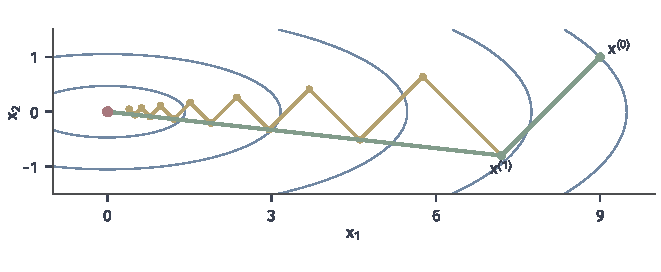
\includegraphics[width=112mm]{figures/05-optimization/02-smooth-optimization/matplotlib/fom-sd-vs-cg/figure.pdf}
  \caption{贯穿例上的精确线搜索路径，蓝色椭圆是等高线。黄色路径是最速下降，绿色路径是共轭梯度法。两者第一步相同，都到达$\bm{x}^{(1)}=(7.2,-0.8)$；共轭梯度的第二步到达最优解（红点），最速下降则继续折返。}
  \label{fig:fom-sd-vs-cg}
\end{BookInlineFigure}

目标不是二次时，两个前提都不存在：没有固定的$\bm{H}$，共轭的定义失去了依托；一般也求不出沿线的精确最小点。\term{非线性共轭梯度法}（nonlinear conjugate gradient method）只保留方向递推的形式，用真实的梯度代替残差，用线搜索代替精确步长。代价是，共轭性一般不再精确保持，有限步终止的结论也不再成立。

\subsection{方向的更新}
\label{sec:fom-ncg-direction}

\paragraph{主要思想}
方法的骨架是
\begin{equation}
 \bm{d}^{(t)}=-\bm{g}^{(t)}+\beta^{(t)}\bm{d}^{(t-1)},\qquad
 \bm{x}^{(t+1)}=\bm{x}^{(t)}+\alpha^{(t)}\bm{d}^{(t)},
 \label{eq:fom-ncg}
\end{equation}
其中$\bm{d}^{(0)}=-\bm{g}^{(0)}$。它只比梯度下降多存一个向量。需要决定的只有两件事：$\beta^{(t)}$怎样算，$\alpha^{(t)}$怎样选。这一小节讨论前者。

在二次目标上，$\beta^{(t)}$可以写成好几种形式，它们彼此相等。写法不同，推广到非线性时就成了不同的算法。从共轭条件出发，要求$(\bm{d}^{(t)})^\top\bm{H}\bm{d}^{(t-1)}=0$，由式~\eqref{eq:fom-ncg}得
\[
 \beta^{(t)}=\frac{(\bm{g}^{(t)})^\top\bm{H}\bm{d}^{(t-1)}}{(\bm{d}^{(t-1)})^\top\bm{H}\bm{d}^{(t-1)}}.
\]

式中含有$\bm{H}$，非线性时无法直接使用。在二次目标上，相邻梯度之差恰好是$\bm{H}$作用在位移上：
\[
 \bm{\delta}^{(t)}:=\bm{g}^{(t)}-\bm{g}^{(t-1)}=\alpha^{(t-1)}\bm{H}\bm{d}^{(t-1)}.
\]

把它代入上式，消去$\alpha^{(t-1)}$，得到只含梯度和方向的表达式：
\[
 \beta^{(t)}=\frac{(\bm{g}^{(t)})^\top\bm{\delta}^{(t)}}{(\bm{d}^{(t-1)})^\top\bm{\delta}^{(t)}}.
\]

精确线搜索使$(\bm{g}^{(t)})^\top\bm{d}^{(t-1)}=0$，并且同样有$(\bm{g}^{(t-1)})^\top\bm{d}^{(t-2)}=0$，由式~\eqref{eq:fom-ncg}得
\[
 (\bm{d}^{(t-1)})^\top\bm{\delta}^{(t)}=-(\bm{d}^{(t-1)})^\top\bm{g}^{(t-1)}=\lVert\bm{g}^{(t-1)}\rVert_2^2.
\]

这样分母化成了$\lVert\bm{g}^{(t-1)}\rVert_2^2$，得到\term{Polak--Ribière--Polyak公式}（Polak--Ribière--Polyak formula，PRP）：
\begin{equation}
 \beta_{\mathrm{PRP}}^{(t)}=\frac{(\bm{g}^{(t)})^\top\bigl(\bm{g}^{(t)}-\bm{g}^{(t-1)}\bigr)}{\lVert\bm{g}^{(t-1)}\rVert_2^2}.
 \label{eq:fom-beta-prp}
\end{equation}

再用线性共轭梯度中相邻梯度的正交性$(\bm{g}^{(t)})^\top\bm{g}^{(t-1)}=0$，分子只剩$\lVert\bm{g}^{(t)}\rVert_2^2$，得到\term{Fletcher--Reeves公式}（Fletcher--Reeves formula，FR）：
\begin{equation}
 \beta_{\mathrm{FR}}^{(t)}=\frac{\lVert\bm{g}^{(t)}\rVert_2^2}{\lVert\bm{g}^{(t-1)}\rVert_2^2}.
 \label{eq:fom-beta-fr}
\end{equation}

两个公式利用的信息不同。FR只看两个梯度的长度，恒为正；PRP还看梯度变化$\bm{\delta}^{(t)}$，它含有两点之间的曲率信息，符号可正可负。在正定二次目标加精确线搜索时两者一致，离开这个条件就是两个算法，下降性和收敛性要分别讨论。

\needspace{6\baselineskip}
\paragraph{变量}
\begin{itemize}
 \item $\bm{x}^{(t)}\in\mathbb{R}^n$：当前点。
 \item $\bm{g}^{(t)},\bm{g}^{(t-1)}\in\mathbb{R}^n$：当前与上一轮的梯度，FR只需要它们的长度平方，PRP需要向量。
 \item $\bm{d}^{(t)}\in\mathbb{R}^n$：搜索方向，算出新方向后覆盖。
 \item $\alpha^{(t)}$，$\beta^{(t)}$：步长与组合系数，用后即弃。
 \item $\varepsilon$，$T$：容差与最大步数。
\end{itemize}

\paragraph{初始化}
令$\bm{g}^{(0)}=\nabla f(\bm{x}^{(0)})$，$\bm{d}^{(0)}=-\bm{g}^{(0)}$，$t=0$。例中
\[
 \bm{g}^{(0)}=(9,9),\qquad\bm{d}^{(0)}=(-9,-9),\qquad\lVert\bm{g}^{(0)}\rVert_2^2=162.
\]

\needspace{6\baselineskip}
\paragraph{每轮更新}
在第$t$轮：
\begin{enumerate}
 \item \textbf{线搜索。}沿$\bm{d}^{(t)}$确定步长$\alpha^{(t)}$。这里先用精确步长，下一小节讨论实际的规则。二次目标的精确步长是
 \[
  \alpha^{(t)}=-\frac{(\bm{g}^{(t)})^\top\bm{d}^{(t)}}{(\bm{d}^{(t)})^\top\bm{H}\bm{d}^{(t)}}.
 \]
 例中第一轮
 \[
  \alpha^{(0)}=\frac{162}{(-9)^2\cdot1+(-9)^2\cdot9}=\frac{162}{810}=\frac15.
 \]

\item \textbf{更新点并读取新梯度。}由式~\eqref{eq:fom-ncg}得到$\bm{x}^{(t+1)}$，并计算$\bm{g}^{(t+1)}$。例中第一轮
 \[
  \bm{x}^{(1)}=(7.2,-0.8),\qquad\bm{g}^{(1)}=(7.2,-7.2).
 \]

\item \textbf{检查停止。}若$\lVert\bm{g}^{(t+1)}\rVert_2\leq\varepsilon$或已达$T$步，输出$\bm{x}^{(t+1)}$。例中第一轮$\lVert\bm{g}^{(1)}\rVert_2^2=103.68$，继续。

\item \textbf{计算系数并更新方向。}按式~\eqref{eq:fom-beta-fr}或式~\eqref{eq:fom-beta-prp}算$\beta^{(t+1)}$，再由式~\eqref{eq:fom-ncg}算$\bm{d}^{(t+1)}$，令$t\leftarrow t+1$。例中第一轮，$(\bm{g}^{(1)})^\top\bm{g}^{(0)}=0$，所以两个公式给出同一值：
 \[
  \beta^{(1)}=\frac{103.68}{162}=0.64.
 \]
 新方向是
 \[
  \bm{d}^{(1)}=(-7.2,7.2)+0.64(-9,-9)=(-12.96,\,1.44).
 \]
 可以核对共轭关系：
 \[
  (\bm{d}^{(1)})^\top\bm{H}\bm{d}^{(0)}=116.64-116.64=0.
 \]

 例中第二轮线搜索，方向导数和曲率分别是
 \[
  -(\bm{g}^{(1)})^\top\bm{d}^{(1)}=103.68,\qquad(\bm{d}^{(1)})^\top\bm{H}\bm{d}^{(1)}=186.624,
 \]
 于是
 \[
  \alpha^{(1)}=\frac{103.68}{186.624}=\frac59,\qquad
  \bm{x}^{(2)}=(7.2,-0.8)+\tfrac59(-12.96,1.44)=(0,0).
 \]
 此时$\bm{g}^{(2)}=\bm{0}$，满足停止条件。
\end{enumerate}

最终得到$\bm{x}^{(2)}=\bm{x}^\star$。二维的二次目标两步到达，这与$n$步终止的结论相符。图~\ref{fig:fom-ncg-direction}画出第二轮方向的合成：新梯度方向$-\bm{g}^{(1)}$与上一方向$\bm{d}^{(0)}$按平行四边形相加，结果恰好指向椭圆中心。

\begin{BookInlineFigure}
  \centering
  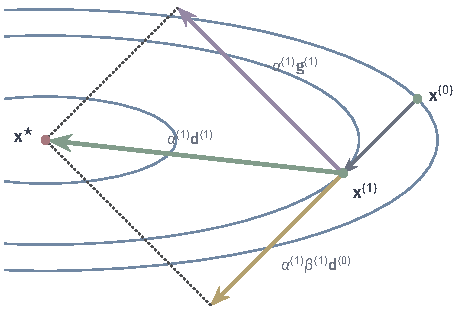
\includegraphics[width=80mm]{figures/05-optimization/02-smooth-optimization/tikz/fom-ncg-direction/figure.pdf}
  \caption{贯穿例第二轮的方向合成，蓝色椭圆是等高线。紫色箭头是负梯度$-\bm{g}^{(1)}$，黄色箭头是上一方向$\bm{d}^{(0)}$乘以$\beta^{(1)}=0.64$，两者都按步长$\alpha^{(1)}=5/9$缩放。绿色箭头是它们的和，从$\bm{x}^{(1)}$直达最优解（红点）。}
  \label{fig:fom-ncg-direction}
\end{BookInlineFigure}

\paragraph{两个公式何时不同}
精确线搜索一旦放宽，即使目标还是二次的，两个公式也立刻分开。在贯穿例第一轮取$\alpha^{(0)}=1/9$，它满足下一小节将列出的线搜索条件，于是
\[
 \bm{x}^{(1)}=(8,0),\qquad\bm{g}^{(1)}=(8,0),\qquad(\bm{g}^{(1)})^\top\bm{g}^{(0)}=72.
\]

这时相邻梯度不再正交。两个系数分别是
\[
 \beta_{\mathrm{FR}}^{(1)}=\frac{64}{162}\approx0.395,\qquad
 \beta_{\mathrm{PRP}}^{(1)}=\frac{64-72}{162}\approx-0.049.
\]

PRP的系数是负的，符号都不同了。对应的方向是
\[
 \bm{d}_{\mathrm{FR}}^{(1)}\approx(-11.56,\,-3.56),\qquad
 \bm{d}_{\mathrm{PRP}}^{(1)}\approx(-7.56,\,0.44).
\]
两者都不再与$\bm{d}^{(0)}$共轭，例如
\[
 (\bm{d}_{\mathrm{FR}}^{(1)})^\top\bm{H}\bm{d}^{(0)}=392\neq0.
\]
方程的形式相同，并不意味着结论相同。

目标非二次时，共轭性的流失更彻底。把贯穿例弯曲一下，取
\begin{equation}
 f(\bm{x})=\frac12x_1^2+\frac92\bigl(x_2-0.1x_1^2\bigr)^2.
 \label{eq:fom-bent}
\end{equation}
这是一条沿抛物线弯曲的山谷，$\bm{x}^\star=\bm{0}$处的Hessian仍是$\operatorname{diag}(1,9)$，系数$0.1$换成零就回到式~\eqref{eq:fom-example}。

图~\ref{fig:fom-ncg-bent}(b)用近乎精确的线搜索运行PRP，并计算相邻方向在当前Hessian下的共轭余弦。它在开始时接近$0.8$，远不是零；直到迭代进入极小点附近、目标接近二次，这个量才逐渐变小。这个二维问题走了$9$步才把梯度降到$10^{-6}$以下，$n$步终止不再成立。

\begin{BookInlineFigure}
  \centering
  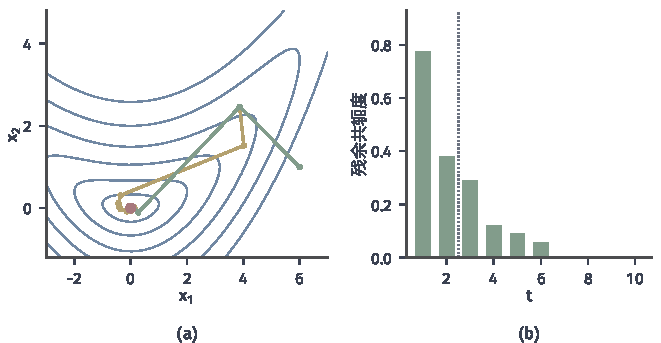
\includegraphics[width=112mm]{figures/05-optimization/02-smooth-optimization/matplotlib/fom-ncg-bent/figure.pdf}
  \caption{弯谷目标~\eqref{eq:fom-bent}上的非线性共轭梯度法，起点$(6,1)$。(a)黄线FR，绿线是把负的PRP系数截断为零的变体PRP+，都采用强Wolfe线搜索（$c_1=10^{-4}$，$c_2=0.4$），画出前$17$步。(b)近似精确线搜索下的PRP，相邻方向的残余共轭度$\lvert(\bm{d}^{(t)})^\top\nabla^2f\,\bm{d}^{(t-1)}\rvert$除以两方向的$\nabla^2f$长度之积，Hessian取在$\bm{x}^{(t)}$；虚线之前是二次目标应该结束的步数。}
  \label{fig:fom-ncg-bent}
\end{BookInlineFigure}

\subsection{线搜索与重启}
\label{sec:fom-ncg-linesearch}

\paragraph{强Wolfe条件}
实际中一般不求沿线精确的最小点。第~\ref{chap:smooth-foundations}章的强Wolfe条件要求步长$\alpha$既满足Armijo条件~\eqref{eq:fom-armijo}，又让方向导数的绝对值变小：
\begin{equation}
 \bigl\lvert\nabla f(\bm{x}+\alpha\bm{d})^\top\bm{d}\bigr\rvert\leq c_2\bigl\lvert\nabla f(\bm{x})^\top\bm{d}\bigr\rvert,\qquad 0<c_1<c_2<1.
 \label{eq:fom-strong-wolfe}
\end{equation}
前一个条件防止走得太远，后一个条件防止走得太近，同时把新点放到沿线函数接近平坦的位置。

贯穿例沿$\bm{d}^{(0)}=(-9,-9)$的一维函数是$\varphi(\alpha)=45-162\alpha+405\alpha^2$，方向导数为$\varphi'(\alpha)=-162+810\alpha$。取$c_1=0.1$，$c_2=0.45$，Armijo条件给出$\alpha\leq0.36$，强Wolfe条件给出
\[
 0.11\leq\alpha\leq0.29.
\]
图~\ref{fig:fom-wolfe}中，$\alpha=1/9$落在区间内，精确步长$1/5$也在区间内。

\begin{BookInlineFigure}
  \centering
  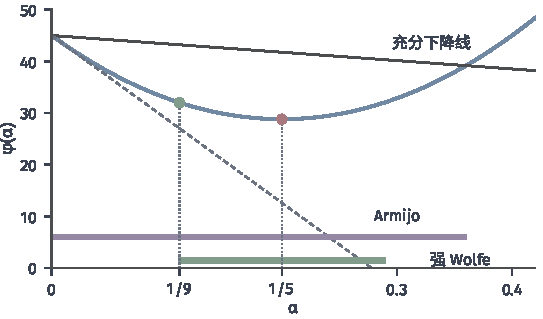
\includegraphics[width=92mm]{figures/05-optimization/02-smooth-optimization/matplotlib/fom-wolfe/figure.pdf}
  \caption{线搜索的可接受区间。蓝色曲线是贯穿例沿$\bm{d}^{(0)}$的$\varphi(\alpha)$，黑色实线是$c_1=0.1$的充分下降线，虚线是$\varphi$在$0$处的切线。紫色线段是Armijo条件接受的区间，绿色线段是再加上$c_2=0.45$的强Wolfe区间。绿点是$\alpha=1/9$，红点是精确最小点$\alpha=1/5$。}
  \label{fig:fom-wolfe}
\end{BookInlineFigure}

\paragraph{FR的下降保证}
方向必须是下降方向，线搜索才有意义。梯度下降中这是自动的，这里却不一定：$(\bm{g}^{(t)})^\top\bm{d}^{(t)}$等于$-\lVert\bm{g}^{(t)}\rVert_2^2$加上$\beta^{(t)}(\bm{g}^{(t)})^\top\bm{d}^{(t-1)}$，后一项可以是正的。精确线搜索让后一项为零；不精确时，强Wolfe条件要限制它的大小。对FR，这需要把$c_2$压到$\tfrac12$以下。

\begin{lemma}[FR方向的下降性]
\label{lem:fom-fr-descent}
设$f$连续可微，每步按强Wolfe条件取$\alpha^{(t)}$，$0<c_1<c_2<\tfrac12$，$\beta^{(t)}$取式~\eqref{eq:fom-beta-fr}，且$\bm{g}^{(t)}\neq\bm{0}$。则对所有$t$，
\begin{equation}
 -\frac{1}{1-c_2}\leq\frac{(\bm{g}^{(t)})^\top\bm{d}^{(t)}}{\lVert\bm{g}^{(t)}\rVert_2^2}\leq\frac{2c_2-1}{1-c_2}<0.
 \label{eq:fom-fr-descent}
\end{equation}
\end{lemma}

\begin{proof}
记中间的比值为$\tau^{(t)}$。对$t$归纳。$t=0$时$\tau^{(0)}=-1$，而
\[
 -\frac{1}{1-c_2}\leq-1\leq\frac{2c_2-1}{1-c_2},
\]
后一个不等号等价于$c_2\geq0$。

设结论对$t$成立，特别地$\bm{d}^{(t)}$是下降方向，线搜索可以进行。由式~\eqref{eq:fom-ncg}和$\beta_{\mathrm{FR}}^{(t+1)}$的定义，
\[
 \tau^{(t+1)}=-1+\frac{(\bm{g}^{(t+1)})^\top\bm{d}^{(t)}}{\lVert\bm{g}^{(t)}\rVert_2^2}.
\]

强Wolfe条件~\eqref{eq:fom-strong-wolfe}给出
\[
 \bigl\lvert(\bm{g}^{(t+1)})^\top\bm{d}^{(t)}\bigr\rvert\leq-c_2(\bm{g}^{(t)})^\top\bm{d}^{(t)}.
\]

除以$\lVert\bm{g}^{(t)}\rVert_2^2$，得到
\[
 -1+c_2\tau^{(t)}\leq\tau^{(t+1)}\leq-1-c_2\tau^{(t)}.
\]

代入归纳假设的下界$\tau^{(t)}\geq-1/(1-c_2)$，左端不小于$-1/(1-c_2)$，右端不大于$(2c_2-1)/(1-c_2)$。由$c_2<\tfrac12$，右端为负。
\end{proof}

用上面$\alpha^{(0)}=1/9$的数据检验。$c_2=0.45$时$\alpha^{(0)}$可接受，引理的区间是$[-1.82,-0.18]$，而
\[
 \tau^{(1)}=\frac{(8,0)^\top(-11.56,-3.56)}{64}\approx-1.44,
\]
确实落在区间内。

\paragraph{FR的全局收敛}
下降方向还不够，还要防止方向几乎与梯度垂直。记$\theta^{(t)}$为$\bm{d}^{(t)}$与$-\bm{g}^{(t)}$的夹角。Wolfe条件带来一个累加估计，它把线搜索的效果转化为对夹角的约束。

\begin{lemma}[Zoutendijk条件]
\label{lem:fom-zoutendijk}
设$f$有下界，梯度$L$-Lipschitz连续，$\bm{d}^{(t)}$都是下降方向，步长满足Armijo条件和Wolfe曲率条件（方向导数至少升到原值的$c_2$倍，$0<c_1<c_2<1$）。则
\begin{equation}
 \sum_{t=0}^\infty\cos^2\theta^{(t)}\lVert\bm{g}^{(t)}\rVert_2^2<\infty.
 \label{eq:fom-zoutendijk}
\end{equation}
\end{lemma}

\begin{proof}
曲率条件是
\[
 (\bm{g}^{(t+1)})^\top\bm{d}^{(t)}\geq c_2(\bm{g}^{(t)})^\top\bm{d}^{(t)}.
\]

两边减去$(\bm{g}^{(t)})^\top\bm{d}^{(t)}$，得到
\[
 (\bm{g}^{(t+1)}-\bm{g}^{(t)})^\top\bm{d}^{(t)}\geq(c_2-1)(\bm{g}^{(t)})^\top\bm{d}^{(t)}.
\]

由梯度Lipschitz，左端不超过$\alpha^{(t)}L\lVert\bm{d}^{(t)}\rVert_2^2$。于是步长有下界
\[
 \alpha^{(t)}\geq\frac{(1-c_2)\lvert(\bm{g}^{(t)})^\top\bm{d}^{(t)}\rvert}{L\lVert\bm{d}^{(t)}\rVert_2^2}.
\]

代入Armijo条件，并用$\lvert\bm{g}^\top\bm{d}\rvert$与$\cos\theta$的关系，得到
\[
 f(\bm{x}^{(t)})-f(\bm{x}^{(t+1)})\geq\frac{c_1(1-c_2)}{L}\cos^2\theta^{(t)}\lVert\bm{g}^{(t)}\rVert_2^2.
\]

对$t$求和，函数值裂项，再用下界，即得结论。
\end{proof}

\begin{theorem}[FR与强Wolfe线搜索]
\label{thm:fom-fr-convergence}
设$f$有下界，梯度$L$-Lipschitz连续。按FR公式迭代，步长满足强Wolfe条件，$0<c_1<c_2<\tfrac12$。若每步$\bm{g}^{(t)}\neq\bm{0}$，则
\begin{equation}
 \liminf_{t\to\infty}\lVert\bm{g}^{(t)}\rVert_2=0.
 \label{eq:fom-fr-convergence}
\end{equation}
\end{theorem}

\begin{proof}
用反证法。设存在$\gamma>0$使$\lVert\bm{g}^{(t)}\rVert_2\geq\gamma$对所有$t$成立。先估计方向的长度。由引理~\ref{lem:fom-fr-descent}，
\[
 \bigl\lvert(\bm{g}^{(t)})^\top\bm{d}^{(t)}\bigr\rvert\leq\frac{\lVert\bm{g}^{(t)}\rVert_2^2}{1-c_2}.
\]

再由强Wolfe条件，并用FR公式把$\beta^{(t+1)}\lVert\bm{g}^{(t)}\rVert_2^2$换成$\lVert\bm{g}^{(t+1)}\rVert_2^2$，展开$\lVert\bm{d}^{(t+1)}\rVert_2^2$，得到
\[
 \lVert\bm{d}^{(t+1)}\rVert_2^2\leq\frac{1+c_2}{1-c_2}\lVert\bm{g}^{(t+1)}\rVert_2^2+\bigl(\beta^{(t+1)}\bigr)^2\lVert\bm{d}^{(t)}\rVert_2^2.
\]

记$c=(1+c_2)/(1-c_2)\geq1$。两边除以$\lVert\bm{g}^{(t+1)}\rVert_2^4$，由FR公式消去$\beta^{(t+1)}$，因此
\[
 \frac{\lVert\bm{d}^{(t+1)}\rVert_2^2}{\lVert\bm{g}^{(t+1)}\rVert_2^4}\leq\frac{\lVert\bm{d}^{(t)}\rVert_2^2}{\lVert\bm{g}^{(t)}\rVert_2^4}+\frac{c}{\lVert\bm{g}^{(t+1)}\rVert_2^2}.
\]

由$\bm{d}^{(0)}=-\bm{g}^{(0)}$，归纳可得
\[
 \frac{\lVert\bm{d}^{(t)}\rVert_2^2}{\lVert\bm{g}^{(t)}\rVert_2^4}\leq\frac{c(t+1)}{\gamma^2}.
\]

再由引理~\ref{lem:fom-fr-descent}的上界，
\[
 \lvert\bm{g}^\top\bm{d}\rvert\geq c'\lVert\bm{g}\rVert_2^2,\qquad c'=\frac{1-2c_2}{1-c_2}>0.
\]
所以
\[
 \cos^2\theta^{(t)}\lVert\bm{g}^{(t)}\rVert_2^2=\frac{(\bm{g}^\top\bm{d})^2}{\lVert\bm{d}\rVert_2^2}\geq\frac{c'^2\lVert\bm{g}\rVert_2^4}{\lVert\bm{d}\rVert_2^2}\geq\frac{c'^2\gamma^2}{c(t+1)}.
\]

右端对$t$求和发散，与式~\eqref{eq:fom-zoutendijk}矛盾。
\end{proof}

定理不要求凸，结论是驻点型的，而且只是$\liminf$，说明有一列子序列的梯度趋于零。它与定理~\ref{thm:fom-gd-nonconvex}的$\lVert\bm{g}^{(t)}\rVert_2\to0$相比更弱，也不给出步数的界。

条件$c_2<\tfrac12$在这里是起作用的：引理的证明里，它让上界保持为负。一旦$c_2\geq\tfrac12$，上述论证不能保证方向下降。

\paragraph{FR的卡顿与PRP的自动重启}
定理保证了极限，却不保证速度。FR有一种典型的卡顿现象。若某一步步长很小，$\bm{g}^{(t)}\approx\bm{g}^{(t-1)}$，那么$\beta_{\mathrm{FR}}^{(t)}\approx1$，新方向约为$-\bm{g}^{(t)}+\bm{d}^{(t-1)}$，几乎沿用了旧方向。旧方向已经效果不佳，下一步又只能走很小的一步，如此延续。

PRP在同样的情形下，分子含有接近零的差$\bm{g}^{(t)}-\bm{g}^{(t-1)}$，于是$\beta_{\mathrm{PRP}}^{(t)}\approx0$，方向自动回到负梯度，相当于重新开始。这就是实践中PRP一般比FR好的原因。图~\ref{fig:fom-ncg-restart}在弯谷上对比了它们。

\begin{BookInlineFigure}
  \centering
  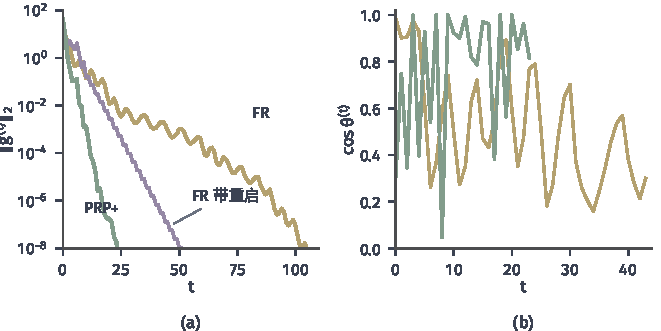
\includegraphics[width=112mm]{figures/05-optimization/02-smooth-optimization/matplotlib/fom-ncg-restart/figure.pdf}
  \caption{弯谷目标~\eqref{eq:fom-bent}上的三种方案，起点$(6,1)$，强Wolfe线搜索$c_1=10^{-4}$，$c_2=0.4$。(a)梯度大小：黄线是FR，紫线是FR加Powell重启（式~\eqref{eq:fom-powell-restart}，$\nu=0.1$），绿线是PRP+。(b)$\bm{d}^{(t)}$与$-\bm{g}^{(t)}$的夹角余弦：黄线FR在后期长时间偏低，绿线PRP+能够多次回到接近$1$的位置。}
  \label{fig:fom-ncg-restart}
\end{BookInlineFigure}

\paragraph{PRP+的下降保障}
PRP的优点有代价。Powell构造过非凸的例子，PRP配合精确线搜索也可能在一组非驻点之间循环，这说明全局收敛不能指望公式本身。这样的反例需要专门构造，证明的细节读者可查阅\scite{math-nocedal2006numerical}。

一个常用的修改是把负的系数截断为零：
\begin{equation}
 \beta_{\mathrm{PRP+}}^{(t)}=\max\bigl\{\beta_{\mathrm{PRP}}^{(t)},\,0\bigr\}.
 \label{eq:fom-beta-prp-plus}
\end{equation}
其含义是：若梯度变化表明上一方向已不再有帮助，就直接扔掉它。贯穿例上$\alpha^{(0)}=1/9$的那一步，PRP+的$\beta$就是$0$，新方向是负梯度$(-8,0)$。

只截断还不够。与FR不同，PRP+在强Wolfe条件下并不自动产生下降方向，因为$\beta$的大小不再受$\lVert\bm{g}^{(t)}\rVert_2^2/\lVert\bm{g}^{(t-1)}\rVert_2^2$限制。已知的收敛定理要求额外的条件：$f$的下水平集有界，梯度Lipschitz，线搜索除强Wolfe条件之外还要保证充分下降，即存在$c>0$使
\begin{equation}
 (\bm{g}^{(t)})^\top\bm{d}^{(t)}\leq-c\lVert\bm{g}^{(t)}\rVert_2^2.
 \label{eq:fom-sufficient-descent}
\end{equation}
在这些条件下可以得到$\liminf\lVert\bm{g}^{(t)}\rVert_2=0$。证明要追踪归一化方向的变化量并作累计估计，篇幅较长，读者可查阅\scite{math-nocedal2006numerical}。这个结论本章没有证明，它依赖的是“PRP+、线搜索与充分下降”三者的组合，缺一项就不能引用。

\paragraph{重启}
非线性情形下，旧方向携带的曲率信息随着地形变化而过期。\term{重启}（restart）就是把方向重置为负梯度，丢弃旧方向。常用的触发条件有三种。

第一种检测方向不再下降：若新方向不满足式~\eqref{eq:fom-sufficient-descent}，立即令$\bm{d}^{(t)}=-\bm{g}^{(t)}$。第二种按周期：每$n$步重启一次，相当于让方向序列按段重新建立。第三种由Powell提出，检测相邻梯度偏离了线性共轭梯度中的正交性：若
\begin{equation}
 \bigl\lvert(\bm{g}^{(t)})^\top\bm{g}^{(t-1)}\bigr\rvert\geq\nu\lVert\bm{g}^{(t)}\rVert_2^2,\qquad\nu\approx0.1,
 \label{eq:fom-powell-restart}
\end{equation}
就重启。

重启并不总是有益的。图~\ref{fig:fom-ncg-restart}(a)的数据是：从$(6,1)$出发，目标梯度$10^{-8}$，FR走了$105$步，加上重启后降到$52$步，PRP+只要$24$步。而对PRP+再加上式~\eqref{eq:fom-powell-restart}，在贯穿起点$(9,1)$上反而从$28$步增加到$52$步，因为PRP+本身已经在需要时自动重置，额外的重启浪费了仍然有用的方向。

下表把变体、线搜索和保证的组合列在一起。引用某个结论时，三列必须同时对应。

\begin{BookInlineTable}
  \centering
  \caption{非线性共轭梯度的常见组合，表中收敛都是$\liminf\lVert\bm{g}^{(t)}\rVert_2=0$。}
  \label{tab:fom-ncg-combos}
  \begin{tabular}{lll}
   \toprule
   变体 & 线搜索与附加条件 & 下降性与收敛\\
   \midrule
   FR & 强Wolfe，$c_2<\tfrac12$ & 下降，定理~\ref{thm:fom-fr-convergence}\\
   PRP & 精确或强Wolfe & 可能循环，无一般保证\\
   PRP+ & 强Wolfe，式~\eqref{eq:fom-sufficient-descent} & 收敛，本章未证\\
   加重启 & 依所用变体 & 保证随所用规则核对\\
   \bottomrule
  \end{tabular}
\end{BookInlineTable}
